\chapter{Language} \label{chap:language}

\begin{flushright}
    \textit{``Quotes are for dumb people who can’t think of anything intelligent to say."}
    \\--- Bo Burnham
%    \textit{``Anything worth knowing is worth writing down."}
%    \\ --- bullseyed723 \footnote{I thought this quote, but also thought it pretentious to quote myself, so I found someone who thought it before me, and so I quote them.}
\end{flushright}

%We knew the problem of semantic disambiguation would be a hard nut to crack, so we sought the outside of the box in pursuit of the holy grail, we let the chips fall where they may but found no one size fits all magic bullet. Afterwards we rolled with the punches, we went back to the drawing board, determined we had bitten off more than we could chew, so we bit a different proverbial bullet, dotted our i's, crossed our t's and saw our glass of cloudy milk was half full of silver lining...
%\footnote{Although technically crossing a t would make an \sout{t}, and dotting an i would make an {\"i}}

%That onslaught of idioms and mixed metaphors is admittedly an extreme example of verbiage, it says almost nothing with the most words possible. A very contrived example of why semantic disambiguation can be notoriously difficult. Semantic disambiguation is one of the biggest open problem in IR research, and also among other fields that relate to Natural Language Processing.

%Idiomatic phrases are specifically intended to have a non-semantic interpretations. Something of a nightmare for semantic disambiguation machines.

%There are many examples of natural language text which are not easily understandable by people. Which is ironic given people are the very people who invented all of the natural languages!

%A naive term matching search engine would identify this very document as being about magic bullets, blood and cats.

%One of the worst culprits of semantic verbiage is academic prose, where academic authors are expected to overuse unhelpfully vague and ambiguous terms like \textit{predominantly} and \textit{utilize}, the understanding is that academic authors should be precise in their use of academic vocabulary, but oftentimes such an excessive level of precision leads to jargon that is incomprehensible even to other academics who share the same academic field as the original author, this over specificity of certain phrases in different contexts leads to further ambiguities in usage, but further to that, this academic style produces long and complex sentences which are unnecessarily verbose, excessively lengthy, overly technical, and can hinder understanding, interpretation, and comprehension, and God forbid lead to miscommunication, sometimes it can almost appear as if an academic author has nothing meaningful to convey, but they persist in producing ludicrously circuitous language in which to say it in, if only to reach some arbitrary word count minimum for some inexplicably vulgar reason. 

Academic prose is one of the worst culprits of semantic verbiage, where academic authors are expected to overuse unhelpfully vague and ambiguous terms within academic documents, with the understanding that the academic readers would expect precision in their use of academic vocabulary, but oftentimes such an excessive level of exactness leads to an impenetrable wall of technical jargon that can become intimidating and incomprehensible even to other expert academics within the same academic field as the original academic author, either through over specificity of specific phrases in different contexts due to the natural semantic shifts of language, fuzzily defined boundaries of prototypical categories, family resemblances of words ---occurring in sense, meaning, usage, and utilization, or simply degradation of language in general, commonly observed in information retrieval research as the ``vocabulary mismatch" problem or the ``term mismatch" problem, which can be immediately seen in the very same academic prose that produces long and complex sentences which are unnecessarily verbose, excessively lengthy, overly technical, and can hinder understanding, interpretation, and comprehension, and God forbid lead to miscommunication, seemingly appearing as though an academic author has nothing meaningful to convey, but they persist in producing ludicrously circuitous language in which to portray it with, if only to reach some arbitrary word count minimum for some inexplicably vulgar reason\footnote{Sorry.}. 

Is it even possible to write academic prose that is not boring?

%Is it even possible for a thesis to not be boring?

% Anyone who writes, should write for everyone. If what you write can only understood by a niche audience, give up, the world doesn't need you. If you are incapable of communicating your ideas in ordinary language you don't understand them well enough yourself, or you just suck at writing. If you can but refuse, you're the kind of pretentious blight that predominantly utilize words like pretentious and blight.

%The University of Otago demands that I conform to \textit{``proper standards of linguistic presentation''}, which is unhelpfully vague. It does not help me, but rather provides themselves with carte blanche to reject my writing if they deem it \textit{improper}, as if that wasn't an arbitrarily subjective judgement. Do rules not need explicit definition?

%Communicating with clarity is already difficult without imposed expectations and limitations, so I choose to write freely, and if I fail to communicate, it is my fault alone.

%I write freely; I write ambitiously; I write for clarity; I write for everyone.

\newpage
\section{Origin of Language}
We cannot be certain of the precise origin of spoken language, as we developed Dictaphone technology well after we developed language. But we can be certain that our ancestors had vocal anatomy \cite{ghazanfar2008evolution}, the tongue, the lips, and most notably the descended larynx that allowed for a phenomenally diverse range of sounds, combined with a primate's proclivity for nonconscious behavioural mimicry, \cite{whiten2000primate, castro2004evolution}. It is safe to assume that any sounds we made were imitated from one generation to the next, a transgenerational game of broken telephone\footnote{This game is known as Chinese whispers in British English and téléphone Arabe in French.}. Monkey see monkey do. Mimicry is not only responsible for the persistence of language, but it could also be responsible for the origin of language. Our ancestors undeniably listened to nature, a crucial skill that aided survival, finding food, and avoiding danger. A contrived example would be the sound of a rattlesnake's tail; the rattling sound is not language but is a threat; it communicates useful information to those who wish to stay safe. Learning to imitate animals would clearly provide an evolutionary advantage. Mimic a prey animal to lure them (e.g.\ duck call), imitate the fierce growl of a predator to intimidate them, or even reproducing the musical melody of a songbird to attract the attention of a cute Cro-Magnon \emoji{graphics/winking-face.png}. Onomatopoeia as the origin of language was first proposed by Darwin in 1871 \cite{darwin1871descent} and is still supported by many scholars today \cite{wood2000human, mithen2006singing, de2017evolution}. These ancient protolanguages did not have meaning per se. They were more like spells that, when incanted, affected the natural world to a survival advantage. 

Modern languages are far from mystical monkey magic, they are precisely defined in two parts, the \textit{words} and their associated \textit{meaning} (Signs and Signified) \cite{chandler2017semiotics, de1989cours}. Linguists have attempted to separate the two sides of this coin to consider them independently, but in everyday usage, they are tightly interconnected like the two sides of a M{\"o}bius strip. Words exist in the real world as representations that can be shared to facilitate communication. The meaning, however, exists only within our minds as abstractions, unable to be observed directly\footnote{A thought unable to be articulated into words is not easily communicated, can you conceive of such a thought?}. A word ---in text or speech--- without any clear meaning is pure nonsense to the listener, akin to the incoherent noise of a foreign language. Sometimes, I stare at printed text until I begin to dissociate, the typeface begins to look strange and unfamiliar, and like an optical illusion I refocus my attention and the words reform as if their presence was normal; as if they were not a complicated hallucination of my mind.

The fluent and literate comprehend a stream of noise\slash lexical symbols into understanding with astoundingly intuitive ease. It is sometimes easy to forget the symbols themselves have no inherent meaning, only the meaning we impose upon them through persistent usage. It is rare to consider the linguistic structures independently unless composing poetic prose with rhythmic rhyming or witty wordplay. We should bear in mind that digital machines see only the lexical form of words, lacking both the cognitive programming and human experience to properly extrapolate meaning the same way we do.



% In communication, we convey our thoughts through symbols. We write and speak, hoping the meaning of our thoughts are understood the way we intended them to be. 



\section{Word Meaning}

Semantics is the branch of linguistics concerning words and their meanings. My personal background in Computer Science (and prior failure of high-school level English) was inadequate preparation for this research. So I began with Routledge textbooks on the English language: \textit{Key Concepts in Language and Linguistics} \cite{trask1999key} and \textit{Philosophy of Language: A Contemporary Introduction} \cite{lycan2018philosophy}. I also read the work of Steven Pinker \cite{pinker2003language, pinker2007stuff, pinker2015words}, Bill Bryson \cite{bryson1990mother}, Robert Fogelin \cite{fogelin2011figuratively}, and Geoffrey Leech \cite{leech2014linguistic}. A significant part of this chapter comes directly from these readings, specifically the linguistic concepts that relate strongly to IR research.

\subsection{Symbol}

The fundamental transactional unit of communication is the symbol, a real-world physical representation that is reproducible. Symbols can take many forms; a guttural grunt, a hand gesture, or a cave wall pictograph. Around 2,000 BCE, Egyptians had about 800 different glyphs \cite{loprieno1995ancient}. At a similar point in history, during the Shang Dynasty, the Chinese had about 4,000 symbols \cite{baxter2014old}. Unicode 13.0 records almost 92,856 symbols for East Asian Languages, but only 3,521 emoji \cite{unicode13}\footnote{Unicode 13.0 has 143,859 registered code-points, 92,856 are dedicated to CJK (Chinese, Japanese, and Korean), that is over 64\%!}. European languages get by with comparatively fewer symbols.

What modern languages have in common is their symbols have both a phonetic and orthographic representation, which is convenient as they can be spoken, written, and easily transformed between these forms. The majority of this thesis will focus on the English language, which has 26 alphabetical letters\footnote{Excluding thousands of Old English words and loan words, like d{\ae}mon, m{\"o}bius, caf{\'e}, and na{\"i}ve.}. A sequence of these letters with some assigned meaning is a word. In this thesis, a \textit{word} is the generalised form, whereas a \textit{term} is a specific word instance found in a document or a search query. For example, ``lollygag'' and ``lollygag'' are the same word but different terms.



Before symbols can be used for communication, to convey meaning, we must reach an understanding of what each symbol symbolises and what each sign signifies\footnote{Unless it's a secret language, then I guess only a select few need to be in the know.}. But what does it mean for a word to \textit{mean} something? There are several distinct kinds of meaning we should first distinguish.

\subsection{Reference}
A word reference is something specific that a word refers to or \textit{points at}. The most common referents are noun phrases and proper names, but broadly anything tangible exists in the real world. For example, \textit{``my cat''}, \textit{``Grumpy Cat''} and \textit{``Mr.\ Bigglesworth''} refer to specific referents. It's also possible for referents to exist in our collective imagination, e.g.\ \textit{Zeus}, \textit{Santa Clause}, or \textit{Capt.\ James T.\ Kirk}, or something in between like \textit{``Zarathustra''}.

% We can also discuss the difference between the historical Jesus and the mythical Jesus.

%, 
% These words act as an indexical or a rigid designator (Kirpke 1970-1980), their meaning is absolute, and unchanging. The meaning of the world ``Gold" is independent on the speakers understanding on Gold. It's still Gold whether the speaker thinks Gold has 79 protons in the nucleus.

\subsection{Denotation}
What a word denotes is no specific real-world thing that can be pointed at but rather a mental schema or concept. It is the literal dictionary definition, some ideal characterization. In the example \textit{``I love cats''}, cats are denoted as a general concept, conjuring thoughts of the stereotypical cat, the maximally typical but hypothetical cat. It may also be thought of as the class of all cats, alive or dead, fictitious or real. This denotation also often entails the superclass of all cat-like things, including both cats and not strictly cats: \textit{Sylvester}, \textit{Tigger}, and \textit{Bastet} being: a cartoon, a cartoon of a plush toy, and the Egyptian God of Protection, respectively.

\subsection{Intension}
Intension is any property or attribute associated with the referent or denoted concept. For example, the word \textit{``cat''} includes the intensions: \textit{``a small domesticated mammal with soft fur, sharp claws, pointed ears, and a long furry tail, often kept as a pet, to catch mice or worship like a god"}. See Figure \ref{dog} for a pictographic explanation. Intensions have varying degrees of association. While we have an understanding of the archetypical cat, it does not need to fulfil every intension to be considered cat-like. A cat without a tail is still a cat.

\begin{figure}[h]
    \centering
    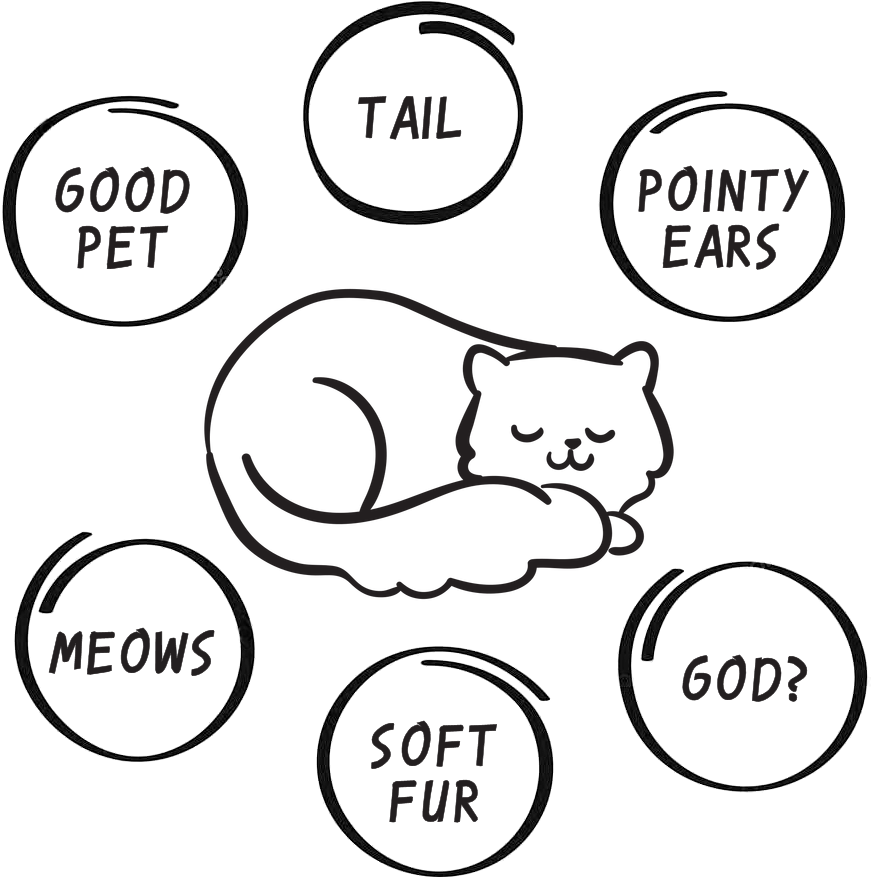
\includegraphics[width=0.6\linewidth]{graphics/cat-intensions.png}
    \caption{Some simple intensions for \textit{``Cat''}.}
    \label{dog}
\end{figure}

\subsection{Connotation}
Many words have an associated emotional colouring, which they have gained through social context and usage. For example, you could describe a person as \textit{slim}, \textit{thin} or \textit{scrawny}. While each of those adjectives describes less body fat than the expected average, they all clearly convey slightly different value judgements. Slim is often associated with attractiveness, thin is neutral, and scrawny is verging on the offensive.

\subsection{Word Sense}
Word sense can be thought of as a word's complete meaning in its entirety. It encompasses any possible reference and denotation; it includes the full set of intensions with all of their associated connotations. Describing a word's sense is often useful when distinguishing between different sets of intensions that could belong to a specific term. For example, the term \textit{``Cats''} has at least four different word senses:

\newpage
\begin{enumerate}
	\item Feline mammals
	\item The Andrew Lloyd Webber musical
	\item Jive talking jazz musicians (1920s slang)
	\item Catalytic converters
\end{enumerate}

Sense 1 and Sense 2 are related, but they are quite distinct concepts (The musical is about, and named after, the animals). Sense 1 and Sense 3 are also etymologically related; jazz musicians have sharp reflexes and are alleged to always land on their feet. Whereas Sense 4 shares no relation with any of the other three, the fact that it too can be referred to via the word ``cats'' is a mere linguistic coincidence, an evolutionary convergence of form. Cat the mammal has historical roots in Proto-Germanic: \textit{``catte''} meaning cat, and catalytic derives from the Greek word \textit{``katalusis''}; Transliterally: \textit{``before-decomposition''}; Translated: initial or initiating action (catalyst).

The meaning of the word \textit{``meaning''} is nebulous, so I will avoid using it where possible. Instead, we will be favouring the more precise word \textit{sense} or \textit{word sense}. All words and terms have an associated word sense unless they are nonsense words, then they, of course, have no sense\footnote{I was delighted to discover the same joke in Wittgenstein's book \textit{Tractatus Logico-Philosophicus} in German. I guess \textit{``great minds think alike"} or rather \textit{``Zwei Dumme, ein Gedanke"}.}.

\subsubsection{Word Definition}
A word's definition is a precise sense, handcrafted by experts for domain-specific nomenclature. The one we are taught in primary school is the biological taxonomy, but every field and activity has its own nomenclature. The word ``brush'' will have a different sense when spoken by a painter, a hairstylist, a makeup artist, a dentist, or an electrical engineer. But they all understand the difference between ``paintbrush'', ``hairbrush'', ``makeup brush'', ``toothbrush'', and ``carbon brush'' (A painter does not usually brush their teeth with a paintbrush). The nomenclature I use every day is that of spoken (and written) English, codified by lexicographers in general-purpose dictionaries. The dictionary is not a superset of all other nomenclatures. It too is domain-specific, the domain of common usage which entails all the idiosyncratic nuances of regional dialects.

A definition ---regardless of the nomenclature--- is carefully designed by experts to include only elements which are both \textit{necessary} and \textit{sufficient} to uniquely identify it. Almost 2,500 years ago, Plato attempted to create a universal definition for ``human''\footnote{Human: The animal who is always in heat.}, which was \textit{``a featherless biped''}. The next morning at the Platonic Academy, Diogenes ---the original cynic and cheeky smarty-pants--- proclaimed \textit{``Behold, Plato's man!''} while holding a plucked chicken aloft. Proving Plato's definition was not sufficient. Featherless may be a necessary condition, but biped may not be as Oscar Pistorius the Blade Runner. The fastest man on no legs, is a human. Although some would argue he is not, not after what he did.
 
 %  usually relative to some context e.g.\ medical definition, biological definition, cosmological definition... the most common is the \textit{dictionary definition}, which is designed for the purpose of general usage, but is prone to the errors induced by ambiguity. 

%The biblical definition of \textit{Jesus} entails the necessary condition \textit{circumcised}, as someone who is not circumcused is necessarily not Jesus, however it's not a sufficient condition, because there are many people who are circumcised that are not Jesus.

%To be a Planet, it is necessary condition to be large enough to become spherical under one's own gravity. But It is not sufficient as Pluto is not a Planet. 

\section{Ambiguity}
If we return to our previous example, \textit{``I love cats''}, we can see that not only is nothing specific being referred to, but also exactly which word sense is denoted is not immediately obvious. Did the author intend to convey a love for the feline mammal, the musical, or some superclass encompassing both? The sentence is ambiguous. An ambiguous statement has two (or more) distinct and sharply precise interpretations. Natural languages are naturally ambiguous. English certainly is.

Ambiguity causes a confluence of senses. Under the term's lexical blanket, word senses may become merged. In this state, distinct words are mistaken for each other, which leads to miscommunication. Within IR research, this phenomenon is known as \textit{Term Conflation}. For example, all of the documents (or websites) containing the term \textit{``apple''} include documents on fruit with crisp flesh and documents about the iPhone company. So to be able to satisfy an information request accurately, a search engine needs to be able to discern the correct word sense for the term \textit{``apple''}, this is to disambiguate the word sense. This process is widely known as Word Sense Disambiguation (aptly named), a specific kind of semantic disambiguation.

\subsection{Vagueness}
Vagueness is often confused with ambiguity. It is, however, a distinct concept. An ambiguous sentence has several precise senses, whereas a vague sentence lacks even one precise sense.

\begin{center}
    \textit{``They will address this issue."}
\end{center}

That sentence is vague. Who is \textit{``they''} referring to? What is the issue? And how exactly will it be addressed? One can be unintentionally vague for many reasons; perhaps one lacks the vocabulary to articulate precise semantics. Or, sometimes, one can be intentionally vague. This is commonly seen in polite speech, where euphemistic phrases are used to avoid the vulgarity of objectionable words. There is also the real possibility of being \textit{Strategically Vague}, where one intentionally obfuscates what they are saying, to be evasive, or to avoid self-incrimination, like the rhetoric of politicians.

\section{Basic Sense Relations}
No word exists in isolation. Each word belongs to an ontology, an entire language, so we should consider how each word relates to all the other words within the language. We can consider the \textit{orthographic similarity} between words, which identifies the similarity of word spelling; the \textit{morphological similarity} considers the word's structure and formation, taking into account root words, prefixes, suffixes...; the \textit{phonetic similarity}, which considers how the words are pronounced. These comparisons encompass etymological derivation, tense derivation, among other more subtle distinctions. 

The most important relationship I am interested in \textit{semantic similarity}, which is known as the sense relation, how similar the respective word senses are, and how dissimilar they are (irrespective of spelling and pronunciation). This allows us to explicitly distinguish between the lexical form of terms from their semantic word sense to help accomplish our ultimate goal of word sense Disambiguation.

%The rest of this chapter is dedicated to the different kinds of identifiable sense relations, including the well known synonymy and antonymy, and also the seemingly less frequent but equally important generonymy and holonymy, as well as several others. 

\subsection{Structure of Sense Relations}

\begin{figure}[b]
    \centering
    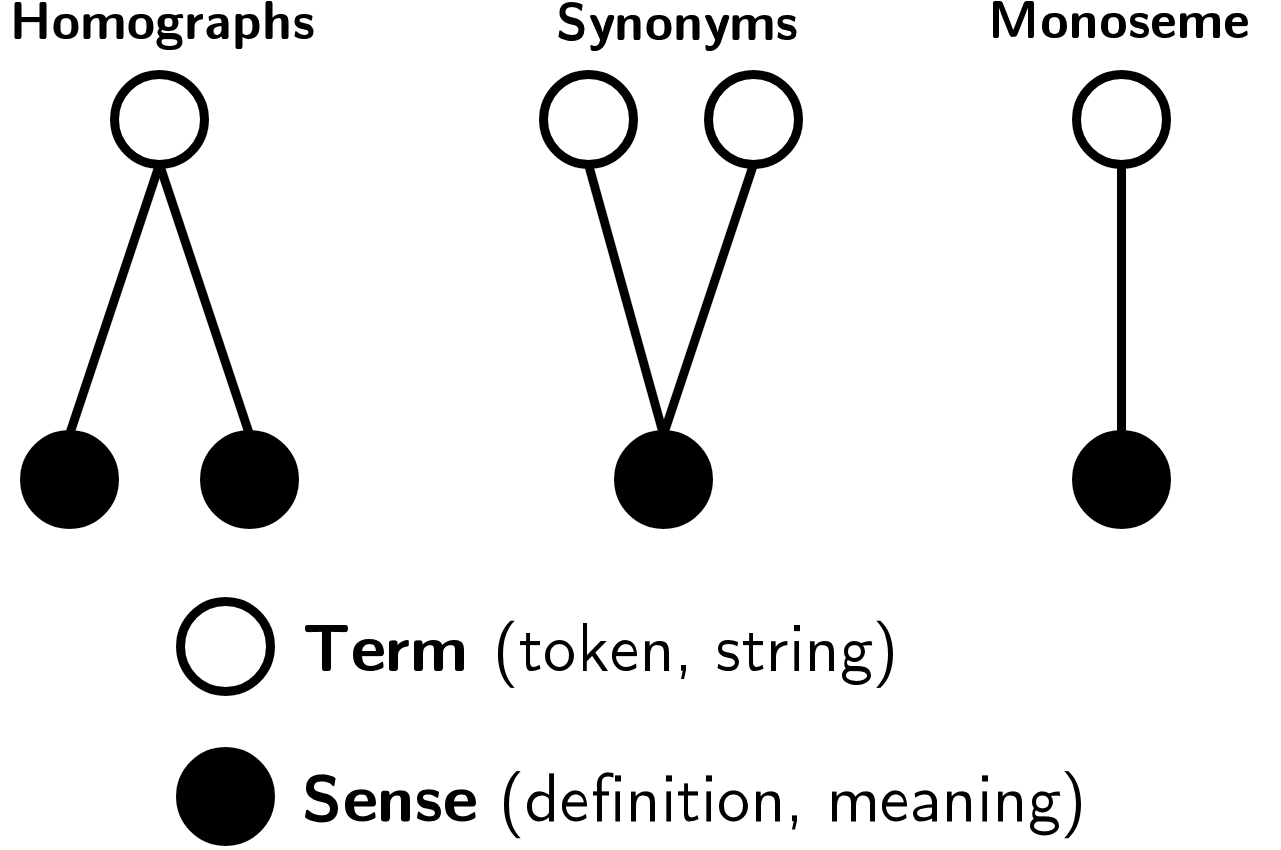
\includegraphics[scale=0.5]{graphics/sense-relations.png}
    \caption{The three basic sense relations.}
    \label{fig:sense-relations}
\end{figure}

% (``with name'')
% (``same name'')
% (``single name'')

There are three basic sense relations shown in Figure \ref{fig:sense-relations}, two of which can cause the plague of vocabulary mismatch. The first is synonymy (with name), where a single concept is associated with two or more different lexical words (e.g.\ ``big'' and ``large''). The second is polysemy (many names), where a single word is associated with two or more distinct concepts (e.g.\ ``cats'' and ``Cats''), The third, which does not concern us greatly, is monosomy (single name), where the concept is associated with one word, and that word is associated with one concept (quite rare), an example of monoseme might be ``\textit{aglet}''. If all words were monosemes, then semantic disambiguation would be trivial. Sadly natural languages were not designed with this in mind. Instead, languages are developed by discordant committees of recently domesticated primates.

%discordant ape like creatures.

\subsection{Homonymy}
Lexical ambiguity is the most simple kind of ambiguity, usually caused by homonymy (same name). We can distinguish between two main classes of homonymy, and in the context of this thesis, we can disregard homophony (same sound) and focus on homographs (same spelling). Homographs are words which have different sense but are spelled identically. Nobody would be surprised if I pointed out that trees, elephants, swimmers, and cars all have trunks because we all know intuitively that there are more things in this world than we have words for them.

\begin{center}
	\textit{``The pilot banked.''}
\end{center}

% My boss was horrified when I pushed my head into his trunks

The above sentence is ambiguous as ``bank'' could mean either an aeronautical manoeuvre or a financial transaction. Since both interpretations are equally valid, it's impossible to discern which single interpretation the author intended.

% \begin{center}
% 	\textit{``I was banking on the plane to bank into the river bank for I had over-insured it with my bank.''}
% 	\\ --- Antanaclasis Contrivance
% \end{center}

\subsection{Polysemy}
Polysemy (many meanings) refers to individual words having several distinct but related senses. It is similar to homonymy in general but differs where the different senses must have some shared association. The distinction between them is tightly linked, and oftentimes harder to spot the ambiguity.

\begin{center}
	\textit{``How to make a chicken salad. \\ Step 1: Make a salad. \\ Step 2: Give it to the chicken''}
\end{center}

The first occurrence of chicken in this sentence is initially ambiguous, referring either to the animal or the meat. This example is supposed to be humorous, and hopefully, you experienced mirth, not embarrassment, upon realizing you had been deceptively led down the garden path. The last sentence is incompatible with the initial interpretation of the first sentence. This forces a cognitive reinterpretation of the semantics. The ambiguity is simultaneously acknowledged and reconciled \textit{...your expectations were subverted, and from whence the humour arose.}\footnote{The young pedant R. Herring would say this after an unnecessary and tedious deconstruction of his own joke--- a despicably self-indulgent man.} %I cannot imagine any more insipidly self-indulgent behaviour.}

Here is a simpler example of the polysemy of \textit{``chicken''}:

\begin{center}
	\textit{``The chicken is ready to eat!''}
\end{center}

The above wordplay cannot be done with most animals in English, as there are usually distinct words for an animal's meat (e.g. beef for cow meat, pork for pig meat). Chicken, the live bird, and chicken the meat are related but clearly different senses. 

There are many different categorisations of polysemy, some more common than others, but all contribute to ambiguity and the vocabulary mismatch problem to varying degrees.

%Homonymy and polysemy aren't mutually exclusive, as shown in the following contrived 

\subsection{Synonymy}
% 
Synonymy (same name) is the relationship between orthographically distinct words that share the same or near-identical word sense. For example, ``big" and ``large" are synonyms, as they are spelled differently, and they share the same sense. Synonyms would be redundant in language usage if there were not more subtle nuanced distinctions that separate them. The degrees of similarity between synonyms are graduated, the most extreme being absolute-synonymy, which is where the words are perfectly identical, and the less extreme being parasynonymy (near name) and partial synonymy \cite{cruse1986lexical}.

\subsubsection{Absolute-synonymy}
Absolute-synonymy is quite rare since it is required that the words could be interchanged in \textit{all} contexts, their difference being only the orthographic spelling. Abbreviations and acronyms can be absolute synonyms, but ``big'' and ``large'' are not absolute synonyms because your \textit{``big sister''} is not the same as your \textit{``large sister''}.

%Which reminds me of this wonderfully understated joke: 

%\begin{center}
%\textit{``Ah, I tell you until I met my wife I always felt incomplete. Now I’m finished.''} 
%\\ --- Norm Macdonald
%\end{center}

\subsubsection{Parasynonymy}
These are words that appear to be absolute synonyms in one nomenclature but are polysemes in another. Mist and Fog are parasynonyms since, in common speech, they both denote a visible mass of condensed water vapour. However, in a meteorological context, there is a precise distinction between how the vapour is formed regardless of density, and the New Zealand Transport Agency makes a precise distinction between how much visual obscurity is caused regardless of the formation\footnote{In meteorology fog is descended cloud, whereas mist forms directly from a nearby water body. In transport safety mist is more transparent than fog, which is more opaque. High-beam headlights are ill-advised when driving through fog as the light reflects back at you.}. So only in common usage would it be appropriate to swap the words mist and fog.

\subsubsection{Partial synonymy}
Partial synonymy is when the similarity relation is not reflexive. That is to say, interchanging the words is only guaranteed to work in one direction. The words ``car'' and ``vehicle'' are partially synonymous because all cars are vehicles, but not all vehicles are cars.  ``Normal'' and ``proper'' are also partially synonymous. People often use those words as if they are interchangeable, however ``proper'' can be used as a pejorative, ``normal'' cannot. Normality is a provable and statistically verifiable state, whereas proper is a value judgement. You cannot label anything as proper just because it is normal.

\begin{table}[h]
    \begin{center}
    %\begin{table}[h]
        \begin{tabular}{|l|lll|}
        \hline
        \textbf{Word} & \multicolumn{3}{c|}{\textbf{Connotations}} \\ \hline
        Conscientious Objector & good & strong & passive \\
        Conchie                & bad  & weak   & passive \\
        Freedom Fighter        & good & strong & active  \\
        Pacifist               & good & weak   & passive \\ \hline
        \end{tabular}
    %\end{table}
    \end{center}
    \caption{The social connotations of anti war}
    \label{tab:psycholinguistic-connotation}
\end{table}

Oftentimes the only discernible difference between synonyms is the social connotation, where the distinction only matters in situations where there is an expected level of politeness or formality, e.g.\ one could describe another who breaks the law as a ``felon'' or a ``crook'', but it would be inappropriate for a Court Magistrate to refer to anyone as a crook in court\footnote{Unless in an unfortunate case of nominative determinism their name was actually ``Crook''}. The connotation entails all the wonderful nuance, the subtle undertones of political and social intention. According to psycholinguistics, words can be connotated in three primary dimensions: Good \& Bad, Weak \& Strong, Active \& Passive \cite{osgood1957measurement}. See Figure \ref{tab:psycholinguistic-connotation} for an example.

The connotations of some the terms in Figure \ref{tab:psycholinguistic-connotation} have evolved over time and are relative to one's own individual political sensibilities. Even seemingly agreed-upon words like ``cat'' can still have a variety of connotations. This is obvious when considering cat lovers against someone who is allergic to cats. The denotation is still the same mammal (e.g\ four legs, whiskers, pointy ears), but the connotation can be quite different.

%Cognitive synonymy

\subsection{Antonymy}
This is one of the more well-known sense relations since it is taught at the primary school level. An antonym (against name) is conventionally thought of as a word whose sense is contrary to another. For example, the words ``left'' and ``right'' are opposite directions so are antonyms of each other. Many antonyms exist on a single dimensional spectrum between two extremes, (e.g.\ \textit{hot, warm, tepid, cold, freezing}). These are known as gradable antonyms. Complementary antonyms have no degrees of gradability but usually express mutually exclusive binary states like ``alive'' and ``dead'', or ``fictional'' and ``factual''. Relational antonymy describes relations between concepts, usually derived from a hierarchy where we have converse pairs like ``boss'' and ``employee'', ``husband'' and ``wife'', or ``parent'' and ``child''. Things get tricky when considering different dimensions an antonym could take from a single word. Is the antonym of ``uncle'' the word ``auntie'' or ``nephew''? Well... both, it depends on the context, whether we are exploring the gender dimension or the ancestral dimension. 

% evening morning
% horizontal vertical

%They are not so easy to group into antonymous pairs, like ``hot'' and ``cold''
%Sometimes these spectrum's have obvious limitations, and sometimes 

% Complementary antonymy each sense is relative to the other, and oftentimes each sense is defined in terms of the other. 

% Interdependence. 

% Unity of opposites. 
% One cannot exist without the other, but they're not strictly contrary.

% material and immaterial
% moral and immoral
% right and wrong
% normal and abnormal

% Parent and child
% Employer and employee
% Teacher and student
% Buy and sell
% Husband and wife
% Predator and prey
% Perpetrator and victim
% Offense and defense
% Slave and master

% politician civilian
% liberal and conservative
% atheist and religious

% chemical and natural
% fictional and factual
% science and supernatural

% Fragile and Robust

% Antifragile


\section{Morphological Changes}

Synonymy and polysemy are the two obvious causes of vocabulary mismatch, but there are a few others we should be aware of that also cause vocabulary mismatch. A word can take many forms, including: tense, case, voice, aspect, person, number plural, gender, and mood. Linguists categorize the different types of morphological change as inflection, derivation, conjugation, and declension. While different word forms are not usually considered synonyms in the conventional sense, through the eyes of a machine, the different forms are orthographically distinct while the sense is very similar. For example, the word sense of ``cat'' is nearly identical to ``cats''.

% When undergoing morphological change the word sense does not change (or only mildly) so these different word forms can be seen as a form of synonymy.

\subsection{Pluralisation}
A word can be inflected to indicate number with either the suffix `s', `es, `ies', or various irregular exceptions. Google's analysis on user behaviour has discovered that in the context of web search, a plural form often indicates whether the user intends to purchase something online \cite{david2006google}, which does make some sense. If the search query was ``digital camera'', the user is likely interested in the concept denoted by \textit{digital camera}, how they work, what they look like, etc. Whereas if the query was ``digital cameras'', it is more likely that the user would be interested in several different types of digital cameras, possibly to compare a variety of them, possibly to determine which kind might best suit their specific needs. That is to say, we can infer that if they need a camera, they might want to purchase one. However, such a long chain of assumptions weakens the inference. Regardless of the justification, plurals can be used to infer what the user's \textit{information need} might be.

% \subsbusection{Inflection}

% inflected forms

% properties or relational information

% present tense, past tense, past participle, and present participle

% Here we added a suffix a very common way to inflect words in English.

\subsection{Derivation}
Derivation is a type of inflection that changes a word's lexical category. One can derive an adjective from a verb, for example ``joyful'' from ``joy''. One can also derive nouns from a verb: ``song'' from ``sing''. In the previous example, a vowel was changed, although changing the suffix is the most common way word derivation occurs.

\subsection{Conjugation and Declension}
Conjugation refers to verb inflection (verb tenses). Languages can have many complicated conjugation rules, especially when accommodating irregularities. Declension is the inflection of everything else, nouns, pronouns, adjectives, determiners etc. Declining a word does not change the lexical category. English only declines nouns to make plurals and also pronouns. German, however, has very complicated declension rules for many words: nouns, pronouns, articles, adjectives, for number, gender, and case.

\begin{center}
\textit{I would rather decline two drinks than one German adjective.}
\\ --- Mark Twain, The Awful German Language
\end{center}

\subsection{Spelling Variation}
An example of absolute synonymy is spelling variation. For example ``colour'' and ``color'', or ``yogurt'', ``yoghurt'', ``yoghourt'', and ``yogourt'' (and when combined with inflection, there are dozens of yogurt variations). Many arise from regional dialects, but on the multicultural, English speaking side of the internet, all of these forms are possible and accepted, which is also useful to know if you are an aspiring internet spelling bee champion.

% indexing process minimal processing, i.e. conversion to lower case, or spelling normalisation

% \subsection{Metaphor}
% Figurative language is common in the poetic arts. When Shakespeare called the world a stage, he did not mean literally but rather figuratively. We would not expect a search query to be written in poetic language. However, metaphor is pervasive in speech, the \textit{foot} of a mountain, the \textit{mouth} of a river. In the world of computing, we commonly use the metaphorical words: \textit{Bootstrap, Branch, Bug, CamelCase, Daemon, Motherboard, Nibble, Pipe, Reboot, Seed, Semaphore, Syntactic sugar, Tree, Trunk, Zombie}. The \textit{World Wide Web} itself is a metaphor for a spider's interconnected web. Within the internet, we also have: \textit{Bookmark, Cloud, Crawler, Firewall, Gateway, Mailbomb, Portal, Surfing}, and the undesirables of the web: \textit{Spam, Trojan, Virus, Worm}. The entire computer user interface is rife with metaphor: \textit{Mouse, Desktop, Clipboard, Attachments, Buttons, Files, Recycle bin, Wallpaper, Windows, Wizard, Zip}. I would also argue that: \textit{Hub, Queue} and \textit{Stack}, are used more figuratively than literally, but that is beside the point. The point is that metaphors sneak into our language far more frequently than we are usually aware of, about once every ten seconds \cite{geary2011other}. However, many of the previous examples would be considered \textit{dead metaphors} rather than the \textit{fresh metaphors} found in poetic prose.

% \subsection{Metonymy}

% Metonyms (change name) are used as replacement words. They refer not to the usual concept but rather some other distinct but associated concept. For example, we might call a New Zealand citizen a ``kiwi'', though they are not literally a flightless bird. \textit{Kiwi} (the bird) and \textit{kiwi} (the people) are polysemous.

% \begin{center}
% 	\textit{``How to make a kiwi salad: \\
% 	Step 1: Make a salad. \\
% 	Step 2: Add kiwi fruit. \\
% 	Step 3: Give it to a kiwi''}
% \end{center}

% The word \textit{Kiwi} (the people) and \textit{New Zealander} are partially synonymous with each other. We should always be aware that a sense relation between words does not exist independently but rather is interwoven within the fabric of language.

% A common basis association in metonymy is \textit{contiguity}, which is when the replacement concept frequently co-occurs with the replaced concept, e.g. kiwi birds, and kiwi people both originate in New Zealand. Other associations which underpin metonymy include metaphor, analogy, visual resemblance and also ellipsis. New Zealand citizens share no salient features with the Kiwi Bird, so referring to them by the metonym ``kiwi'' is not metaphorical or analogical resemblance.

% \subsection{Proper Nouns}
% Metonymy is especially prevalent when referring to a specific referent: \textit{a person}, \textit{place} or \textit{thing}\footnote{but what is a place? but a thing large enough to stand on, and what is a person but a thing that can talk back.}. Some \textit{things} become so widely known that they gain an epithet, an attribution provided after the standard name, as in Alexander \textit{the Great}. Antonomasia is when the phrase excludes the referent's standard name, e.g.\ ``The King of Pop'' or ``The Big Apple'', i.e.\ a metonym. Antonomasia also includes aliases, pseudonyms and nicknames like ``George Orwell'' being the pen name of ``Eric Arthur Blair", ``Father of Computer Science'' referring to the great Alan Turing.

%, or ``Laughter Critic'' referring to Plato\footnote{Plato thought laughter to be an irrational emotional outburst. He also thought laughing itself to be evil, to take delight in an other's self-ignorance --- and that malice is morally objectionable}.

% Many of us understand these metonyms intuitively; they are, after all, used primarily for famous referents. And if we are unaware of some specific nickname, there is certainly someone nearby who can help elucidate these for us. A machine has no such affordance.

%The distinction between homonymy and polysemy becomes blurred henceforth
%Not strictly a kind of polysemy, although we are still discussing words with related senses.

% \subsubsection{Eponymy}
% An eponym is a proper noun named after a specific historical person or region, usually the person who discovered or invented the noun's referent or region of origin. Common things which are eponymously named include body parts, diseases, laws, and food.

% \begin{center}
%     \textit{Moore's Law, Zipf's Law, Turing Test}
    
%     \textit{Reuben Sandwich, Roman Numerals, Champagne...}
% \end{center}

% And since proper nouns can be legally copyrighted, we can now distinguish whether a referent is legally authentic or a cheap imitation. Is sparkling wine made \textit{via methode champenoise} but outside of the Champagne wine region even real champagne? Are Roman numerals written outside of Rome even real numbers? 

% \subsubsection{Generonymy}
% Legally trademarked names are frequently used out of their legal context, to the point at which they lose their legal definition. This is known as Trademark erosion. When searching for something on the internet, we often use the verb ``google'', we refer to inflated cushioning as ``Bubble wrap'', and my mother will never not refer to any video game console as ``the Nintendo''. Sometimes these words become so common in speech they become considered generic. It is possible that the trademark protection will be legally dropped, as in Motorola's previous trademark ``Flip Phone'' or Apple's ``App''.

% the Lego company trying to enforce the plural form is lego not legos 

%Referring to a plush toy as a cat, is a kind of ..., the reference is through resemblance, a kind of visual metaphor. The soft toy still shares many salient or prominent features with cats.

\section{Ontological Relations}

So far we have only discussed attributes of a word and binary relationships between words. However, words do not exist independently but rather interwoven within the fabric of language, so let us quickly discuss hierarchical relationships and indirect relationships before moving on to the next chapter.

\subsection{Meronymy and Holonymy}

Objects in the real world can be broken down into constituent parts, and sometimes we might refer to the whole of an object from one of its parts. For example, a car could be referred to simply as ``wheels''. This is known as meronymy (part name), a specific type of partial synonymy. This language feature is often used to shift the reader's focus to what is most relevant for the situation. For example, if I had to feed several hungry people, I might refer to them as ``mouths'' to feed. There are several ways in which something could be considered a part of something else. Table \ref{meronymyholonymy} shows the most common types.

% \begin{center}

\begin{table}[h]
\centering
\begin{tabular}{|l|l|l|}
\hline
\textbf{Type}  & \textbf{Meronym}   & \textbf{Referent}    \\ \hline
Structure      & wheels  & Vehicle with wheels \\
Characteristic & fizzy   & Carbonated beverage \\
Substance      & ice     & Cube made of ice   \\
Containment    & wine    & Glass filled with wine \\ \hline
\end{tabular}
\caption{Different types of Meronyms}
\label{meronymyholonymy}
\end{table}

% \end{center}

%Containment     Pint            Pint of beer
%Membership      Otago Daily Times	a person who works for the ODT

The inverse of meronymy is holonymy (whole name), which occurs when denoting or referring to a constituent part from its whole. For example, being ``interviewed by the Otago Daily Times'' does not mean the entire company conducted the interview, more likely by a single employee or representative. 

% Perhaps this is an elliptical expression, or possibly both?

%Some examples of meronymy or holonymy may be caused by ellipsis. We do not care so much how the language evolved each particular phrase, but rather how they relate to each other now.

\iffalse
Wheels	    Car						            Part			precise
Blade		Sword						        Part			precise
Boots		Soldiers					        Part			precise
Toast		toasted bread					    Part			precise
Fizzy 		carbonated beverage				    Part			precise
Bubbly		sparkling wine					    Part			precise
Redhead	    a person who has red coloured hair		Part	    precise
Suit		a business person who wears a suit		Part		precise
Glasses	    spectacles made of glass			Substance		precise
Rubber	    Latex rubber condom				    Substance		precise
Ice		    ice cubes					        Substance		precise
Chalk		Stick of chalk					    Substance		precise
Paper		newsprint paper
\fi

\subsection{Hypernyms and Hyponyms}

We can categorize words by their degree of specificity and generality. In information science, an ontology is a structured hierarchy identifying categorical relationships between concepts, a taxonomy of words. The top-level or root of any ontology is the most general and includes more schematic or abstract concepts. The lower levels include more specific and detailed concepts or instances. This kind of data structure should be reminiscent of the knowledge base representations mentioned earlier and our mental model of word associations.

%The intermediate levels are 

\begin{figure}[h]
    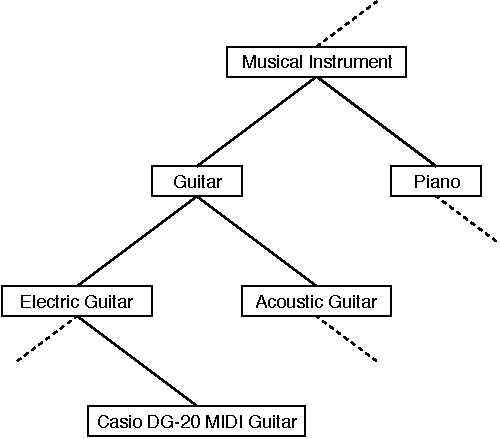
\includegraphics[width=0.8\linewidth, left]{graphics/level_of_specificity.pdf}
  \caption{Simple Ontology Example}
  \label{fig:ontology}
\end{figure}

\iffalse
\begin{table}[h]
\begin{tabular}{|l l|}
\hline
Physical object & \textit{Most generic} \\
Musical instrument & \\
Guitar & \\
Electric Guitar & \\
Casio DG-20 MIDI Guitar & \textit{Most specific} \\
\hline
\end{tabular}
\end{table}
\fi

The level at which we refer to something is strongly dependent on the current context. When in a music shop, it would be important to distinguish \textit{precisely} which musical instrument you might refer to. But when in my bedroom you may be more general, as ``the guitar'' could only refer to my 3/4 size acoustic guitar that I bought, fully intending to learn how to play it one day. The convention is to adhere to the Level of Usual Utility \cite{brown1958shall}, one should not be annoyingly vague nor cumbersomely explicit. One should convey strictly enough information for the situation. If one were looking on the internet to purchase a guitar, the level of specificity would be important.  

%Superordinate level
%Intermediate level
%Suborinate level
%superordinate,


%hierarchical structure

The categorical relationships described above are known in linguistics as hypernymy and hyponymy. A hypernym (over name) refers to a more general term, and a hyponym (under name) refers to a more specific term. This is another kind of partial synonymy we mentioned earlier. It is sometimes considered a \textit{type-of} relationship, distinct from the other class of partial synonymy (meronymy and holonymy), which are considered a \textit{part-of} relationship. Another distinction is that Hypernymy and Hyponymy are transitive relations, so if a Casio DG-20 is a type of guitar, and a guitar is a type of musical instrument, this allows us to infer that Casio DG20 is a type of musical instrument by the rule of transitivity.

In everyday speech, one might make a breakfast request of \textit{``eggs on toast with a glass of milk''} from a caf{\'e}, and a maliciously compliant genie who works at the caf{\'e} could serve \textit{fish eggs} and \textit{giraffe milk}. The breakfaster likely intended \textit{chicken eggs} and \textit{bovine milk} as they are the most commonly egg and milk products consumed in our society, which is why we can refer to them through their respective hypernyms ``milk'' and ``eggs''. Academics and suits of marketing tend to use hypernyms to make products sound more sophisticated than they actually are. For example, a toothbrush might be referred to through its hypernym ``dental cleaning tool'', or even calling a web search engine a ``digital information retrieval system''. Such a level of over-specificity is redundant and prevents clear and concise communication.

Now that we have established an understanding of how words relate to each other within an ontology in the next chapter we will investigate various methods of modifying search queries to improve document retrieval. The method we are most interested in are those which use a semantic ontology to inform this modification process.